% ---
% Arquivo com a Introdução do Trabalho de Conclusão de Curso do aluno
% Daniel Noriaki Kurosawa
% da Escola Politécnica da Universidade de São Paulo
% ---

	\chapter*[Introdução]{Introdução} %(exemplo de capítulo sem numeração, mas presente no Sumário)
	\addcontentsline{toc}{chapter}{Introdução}
	Em muitas situações de risco \cite{uses-robot} é preferível hoje o envio de robôs a humanos devidonecessitamos interagir com um ambiente remoto e\par
	
	
	Braços robóticos possuem uma ampla gama de aplicações,substituindo seres humanos em tarefas em locais de difícil acesso, repetitivas, ou de alta periculosidade, indo seu uso desde o desarmamento de bombas ao uso em missões espaciais\cite{uses-arm}, passando por processos industriais\cite{uses-robot}.\par
	
	 Entretanto, muitas das abordagens para sua operação continuam complexas e anti-intuitivas  necessitando do uso de artifícios como controles remotos\cite{datasheet-caliber} e joysticks\cite{joystick}. \par
	 
	 Uma segunda linha de pensamento tenta se aproveitar de semelhanças físicas entre o corpo humano e o braço robótico e faz uso, por exemplo, de sensores \cite{wearable} e marcadores\cite{tracker-based} presos ao corpo. Entretanto, essas abordagens podem se provar incomodas ou restritivas em relação à movimentação do usuário devido por exemplo, a ocultação de um marcador ou a rigidez de um sensor vestível.\cite{kinect-based}\par 
	 
	 Uma solução para essas restrições é o uso de tecnologia de rastreamento visual sem marcadores, que permite que o usuário não mais se preocupe com as restrições de movimento impostas, tornando o controle mais natural.\cite{kinect-based} \par 
	
	 Paralelamente a operação do braço robótico, este trabalho estuda o uso de um sistema de imersão visual através do uso de um óculos realidade virtual por rastreamento dos movimentos da cabeça do usuário e um sistema de câmeras estereoscópicas ao projeto, com a finalidade de criar uma experiência imersiva ao usuário (......)\par 
	
	 
	
	
	
	
	\begin{figure}[ht!]
		\caption{\label{fig_diagrama}Diagrama do projeto}
		\begin{center}
		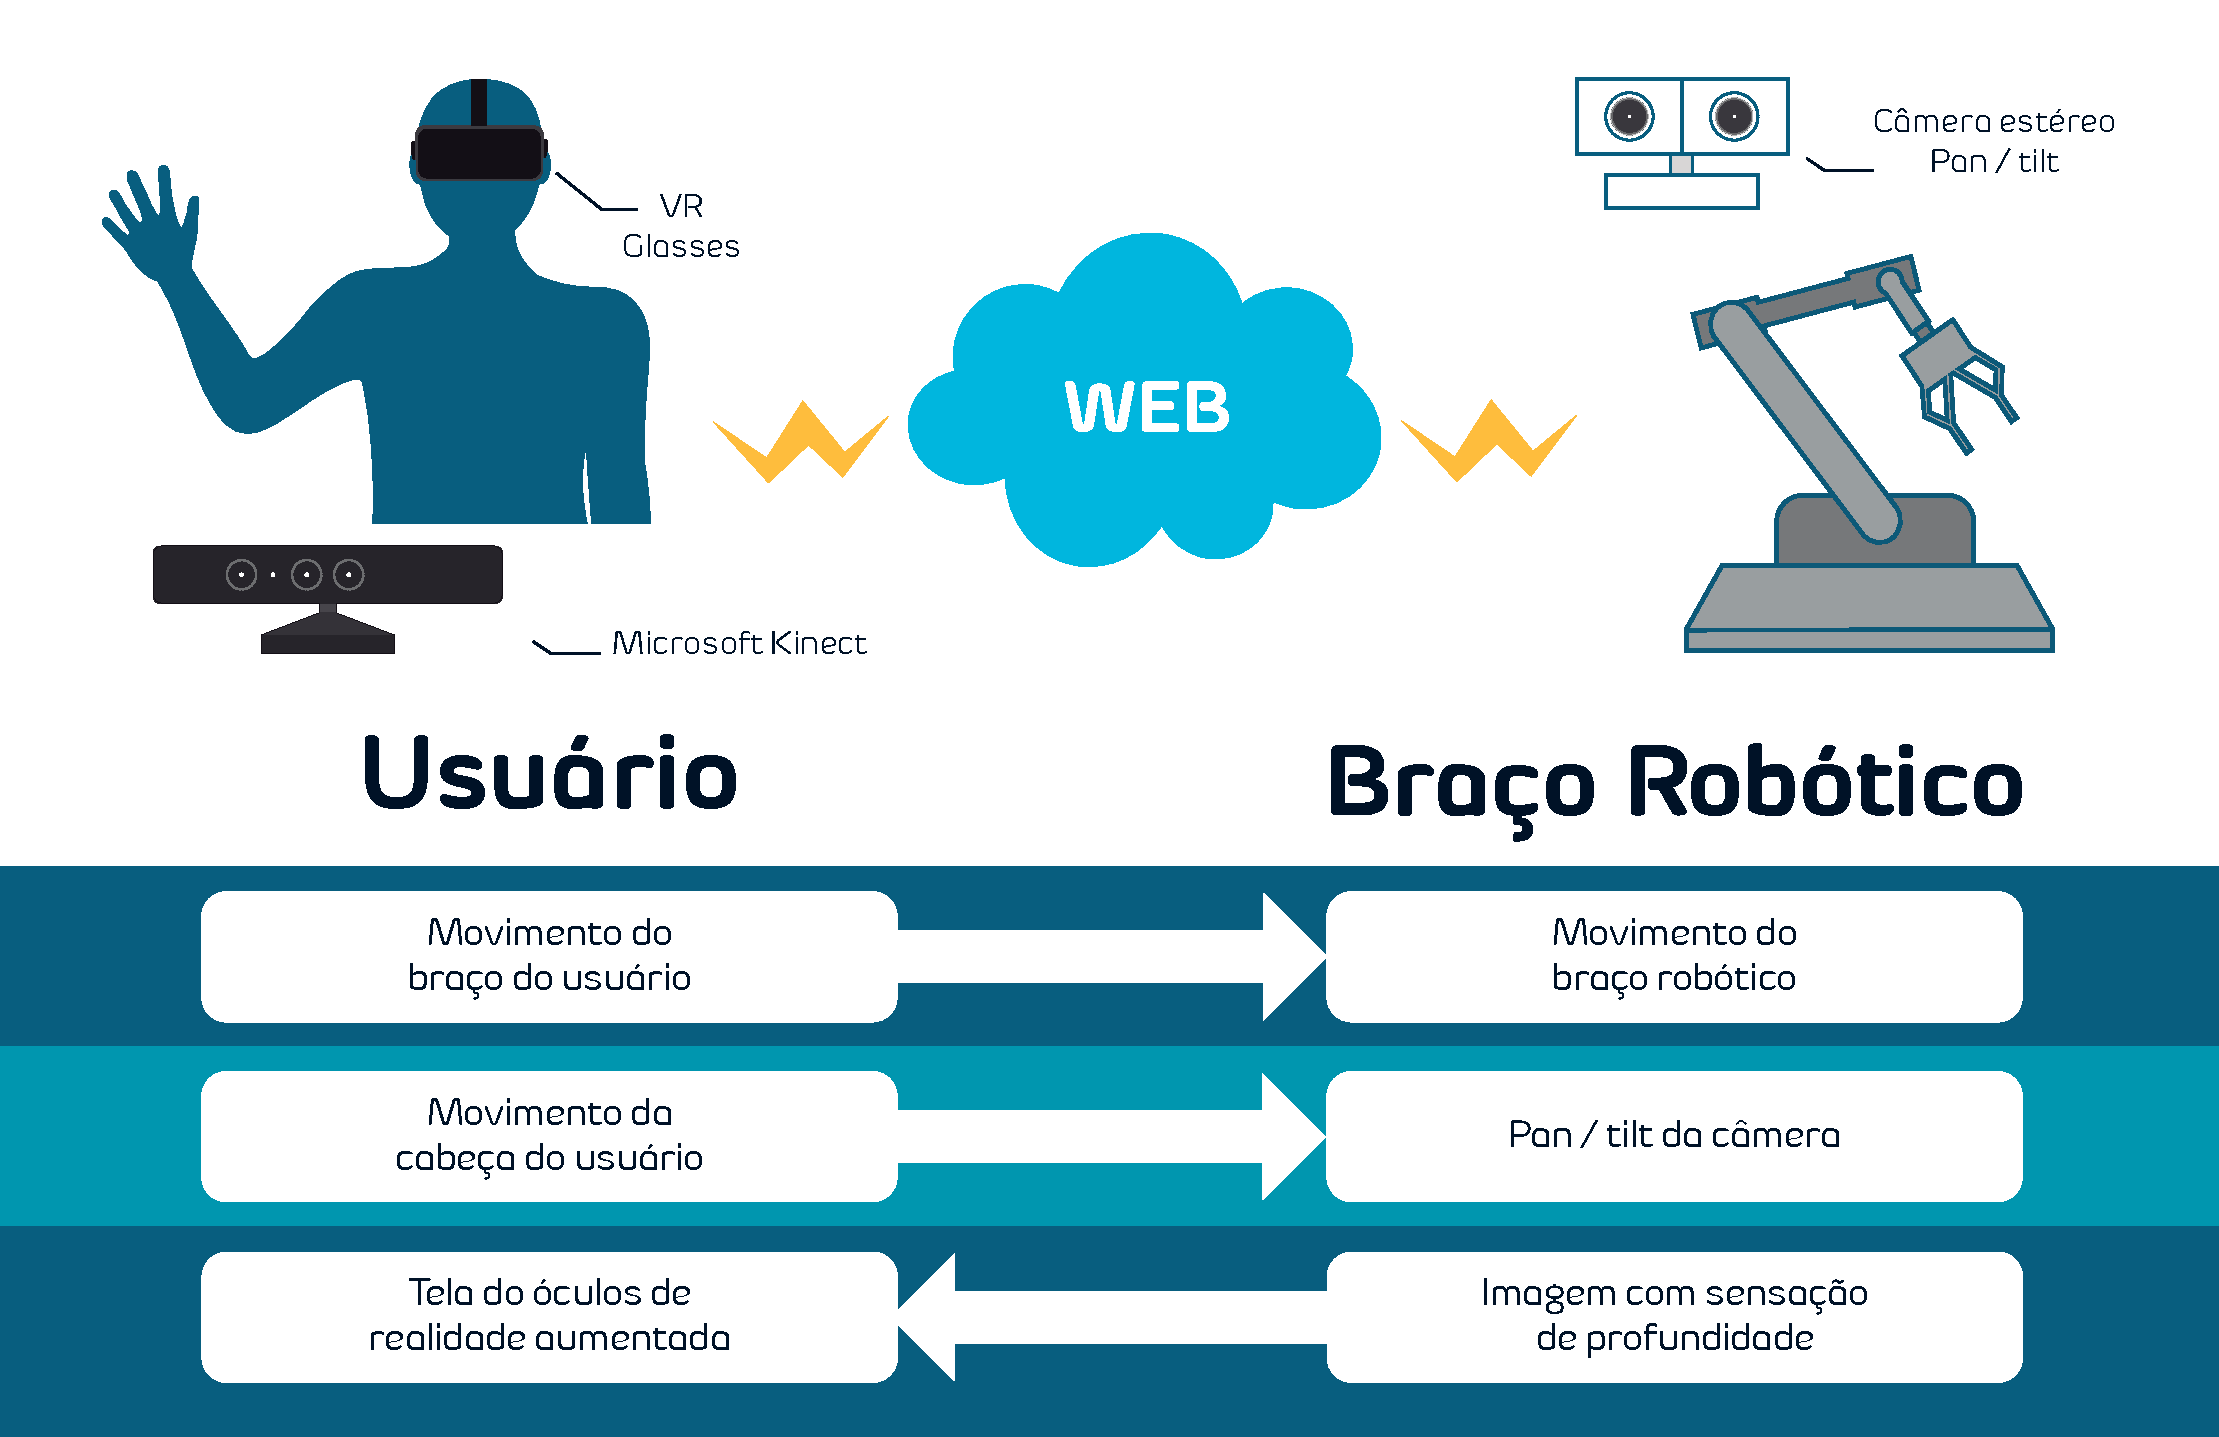
\includegraphics[width=\textwidth]{projectchart.pdf}	
		\end{center}
		\legend{Fonte: Autor}
	\end{figure}
	

	
	\section*{Motivação}\label{sec-motivacao}
	
	Este projeto tem como antecedentes experiências com comunicação via luz visível. Criadas no contexto de uma disciplina de laboratório de processadores, as principais motivações foram a maior eficiência energética da VLC, bem como a diminuição de interferência com ondas de radiofrequência. No entanto, estas experiências esbarraram em desafios, principalmente relacionados à falta de um padrão de comunicação e de componentes adequados. Além disso, houve problemas relacionados à capacidade de processamento do microcontrolador utilizado, o que é consequência de um levantamento de requisitos incompleto.
	
	Sendo assim, este projeto surge como um amadurecimento dos objetivos anteriores. Neste segundo momento, foi escolhida uma norma que atendesse às expectativas de implementar comunicação por luz visível de forma eficiente. O padrão IEEE 802.15.7 apresenta a vantagem de ter se completado em dezembro de 2011 e já ter se consolidado entre companhias e grupos industriais que formam o Consórcio Li-Fi. Além disso, o rigor metodológico é uma das preocupações centrais do novo trabalho, o que inclui um refinamento na maneira de definir os requisitos do sistema.
	
		\section*{Ideias iniciais e alternativas do projeto}\label{subsec-iniciais}
	
	Inicialmente, a pesquisa inicial tratou os seguintes temas:\par
	
	
	\begin{itemize}[noitemsep]
		\item Geração de trajetória para braço robótico usando Microsoft Kinect;
		\item Captura de movimentos usando giroscópio;
		\item Algoritmos anti-drifting de giroscópio;
		\item Captura de imagens estereoscópicas em tempo real;
		\item Arduino;
		\item Raspberry Pi;
		\item Particle Photon;
		\item Internet of Things;
	\end{itemize}
	As ideias iniciais continham premissas que envolviam o uso de redes neurais para o controle do braço mecânico, utilizando um controlador ANFIS-PID para o controle dos motores, chegando a ser testado.\par
	Posteriormente, em virtude de limitações de memória do hardware e a complexidade adicionada ao projeto, os algoritmos de redes neurais foram excluídos do escopo do projeto.
	O formato final é tratado na seção seguinte.
	\section*{Objetivo}\label{sec-objetivo}

Este estudo se propõe realizar o controle de um braço mecânico simplificando seu método de entrada de comandos sem elevar significativamente seu custo de projeto.\par
Colocado este objetivo, uma primeira preocupação do projeto é quanto a sua adaptabilidade. Para que o projeto possa ser aplicado a uma ampla gama de finalidades, o projeto foi subdividido em pequenos subprojetos, que podem ser utilizados com independentemente. Para isso será utilizado um ao realizar a comunicação em tempo real através da internet, introduzindo o conceito de Internet of  Things (IoT) ao projeto. 
Serão levadas em considerações parâmetros como a robustez, taxa de transmissão de dados, custo da transmissão de dados, segurança do meio de comunicação, sendo necessária uma análise usando Architecture Tradeoff Analysis Method (ATAM) .
Uma vez que o controle é realizado a distancia, este trabalho se propõe a implementar um sistema de câmeras imersivas estereoscópicas, em que a movimentação de duas câmeras instaladas próximas ao braço robótico será controlada pela movimentação da cabeça do usuário, sendo as imagens assim obtidas transmitidas uma à cada olho do usuário através de óculos visores, provocando a sensação de profundidade.